\chapter{Code-mixing in the prepositional phrase}\label{PP}

This chapter\footnote{This chapter is based on an earlier publication, see \citet{reif-robinson}.} examines patterns of insertional code-mixing in the prepositional phrase. This syntactic context is one the most frequently reported loci for code-mixing: a speaker can switch the language either at the boundary of the prepositional phrase (cf. \citealt[314]{bentahila-davies-1983}; \citealt[271, 315]{boumans-syntax-1998}; \citealt[757]{clyne1987}; \citealt[169]{haust-codeswitching-1995}; \citealt[310]{pfaff-constraints-1979}; \citealt[208, 221--224]{treffers-daller-mixing-1994}) or within the prepositional phrase, i.e., between the preposition and the noun phrase (\citealt[315]{bentahila-davies-1983}; \citealt[602]{poplack-sometimes-1980}; \citealt[310]{pfaff-constraints-1979}; \citealt[173, 178]{stenson-1990}). If we restrict our attention to insertional code-mixing, we can subsume these phenomena under the concept of insertion. Either a prepositional phrase or a noun (phrase) is inserted from one contact language into a clause framed by the other contact language. In other words, prepositional phrases involved in code-mixing are either inserted or mixed. These mixing patterns are also regularly found in Russian-German bilingual speech in Germany as documented in my corpus. Despite frequent mention of these patterns in the literature, systematic investigations of  variation in this syntactic context are still missing from research, let alone studies uncovering the factors driving this variation. The purpose of this chapter is therefore to describe and account for variation in code-mixing in the prepositional phrase as observed in my Russian-German data. In doing so, I will take a usage-based perspective on the examined patterns and view this variation as an outcome of usage-based factors, which include frequency of (co-)occurrence and repetition of words in discourse.

The structure of the present chapter will be largely identical to the structure of Chapter \ref{NP}. First, I will briefly outline two accounts of insertion: Carol Myers-Scotton's Matrix Language Framework and Ad Backus' unit hypothesis (they are given a detailed presentation in Chapter \ref{CM}). The next section will describe inserted and mixed prepositional phrases in my corpus of Russian-German bilingual speech. Section three will be concerned with factors that influence switch placement in the prepositional phrase. In the subsequent section, I will report the results of the statistical analysis testing these factors and their contribution to the scrutinised variation. Finally, I will summarise the results of the study and put them in the broader perspective of usage-based linguistics.

\section{Previous accounts of mixing in the prepositional phrase}
Although code-mixing in the context of the prepositional phrase is widely reported in bilingual speech involving various language pairs, few scholars have attempted to elucidate the factors underlying the choice between placing a switch within the prepositional phrase and switching the language at the phrase boundary. Such variation has been of particular interest to the Matrix Language Framework (MLF) model \citep{myers-scotton-duelling-1993,myers-scotton-contact-2002}. As has been laid out in the previous chapters, the principal tenet of this model is that one of the languages in contact provides the core clause structure, whereas the role of the other language is restricted to the supply of lexical items. The structure of a bilingual clause is hence analysed by determining the division of labour between the involved languages. The language responsible for the core clause structure is labelled as the matrix language (ML), the other, dominated language is the embedded language (EL) \citep[75--119]{myers-scotton-duelling-1993}. As a result of this asymmetry, embedded-language content morphemes such as nouns are inserted into constituents organised by the matrix language to form mixed constituents. Other lines of research refer to this situation as insertional code-mixing (cf. Chapter \ref{CM}). For example, in (\ref{ex:5:1}), the prepositional phrase consists of the Croatian preposition \textit{u} `to' and the mixed constituent \textit{city-ju} `city-\textsc{acc.sg.f}. The mixed constituent emerges because the English noun \textit{city} receives the Croatian inflectional suffix \textit{-ju} of the accusative case, which is assigned by the preposition \textit{u} `to' to its complement.
	
\ea
\label{ex:5:1}
Croatian-English \citep[203]{hlavac-second-generation-2003}\\
\gll i {iš-l-i} {smo} {u} {\textit{city}-{ju}}\\ 
	{and} go-\textsc{ptcp-pl} be.\textsc{prs.1pl} to {}-\textsc{acc.sg.f}\\
\glt `\dots{}and we went to the city\dots' 
\z

\noindent Embedded-language noun stems sometimes lack matrix language case markers, as in (\ref{ex:5:2}), where the noun \textit{city}, again preceded by the Croatian preposition \textit{u} `in', does not take the required inflectional suffix of the locative case and remains bare.

\ea
\label{ex:5:2}
Croatian-English \citep[202]{hlavac-second-generation-2003}\\
\gll {ja} {bolje} {vol-im} {bi-ti} {u} \textit{city} \\
	{I} more like-\textsc{prs.1sg} be-\textsc{inf} in {}\\
\glt `\dots{}I like more to be in the city\dots{}'
\z

\noindent In bilingual speech, prepositional phrases consisting of a matrix language preposition and a mixed constituent, as in (\ref{ex:5:1}), and those consisting of a matrix language preposition and a bare embedded-language noun, as in (\ref{ex:5:2}), alternate with prepositional phrases containing only embedded-language morphemes. Such constituents are covered by the umbrella term “embedded-language islands”. Under this model, the English prepositional phrase \textit{down the stairs} in (\ref{ex:5:3}) is analysed as an embedded-language island.

\ea
\label{ex:5:3}
Croatian-English \citep[227]{hlavac-second-generation-2003}\\
\gll {\dots{}i} {jedan} {dan} {ja} {sam} {pa-o} \textit{down} \textit{the} \textit{stairs} {i} {jedan} {je} {bi-o\dots{}}\\
	{and} one day I be.\textsc{prs.1sg} fall-\textsc{ptcp.sg.m} {} {} {} and one be.\textsc{prs.3sg} be-\textsc{ptcp.sg.m}\\
\glt `\dots{}and one day I fell down the stairs and one was\dots{}'

\z

\noindent \citet{myers-scotton-matching-1995} explain the appearance of embedded-language islands in code-mixed utterances by mismatches in the grammatical information contained in lemmas, which are defined as entries in the mental lexicon underlying lexical items. Following their view (ibid., 1008--1014), lemmas represent grammatical information at three levels: (\textit{i}) lexical-conceptual structure (semantic/pragmatic features), (\textit{ii}) predicate-argument structure, and (\textit{iii}) morphological realisation patterns. The lack of congruence at one of these levels between the relevant embedded-language lemma and its matrix language equivalent can result in the emergence of an embedded-language island. According to \citet[][227]{hlavac-second-generation-2003}, the embedded-language island \textit{down the stairs} in (\ref{ex:5:3}) is produced because the content morpheme \textit{down} ``for most of its uses in English $[\dots{}]$ is non-congruent to any Croatian content morpheme equivalent''. That is, the embedded-language island emerged because of lacking congruence in the lemmas involved at the level of lexical-conceptual structure. At the same time, \citet[258]{deuchar-congruence-2005} contends that semantic/pragmatic differences between lemmas, as in (\ref{ex:5:3}), can motivate the appearance of specific switches, but only grammatical congruence determines the possibilities for code-mixing. While in Chapter \ref{NP}, devoted to the analysis of mixing in the adjective-modified noun phrase, I considered the constituent's internal structure and its word-order pattern as crucial features pertaining to congruence in the realisation patterns, in the case of prepositional phrases, it is congruence at the level of adposition that is relevant in the first place. Different realisation patterns of adposition indeed seem to regulate the occurrence of embedded-language islands structured as adposition phrases in certain language pairs. For instance:

\ea
\label{ex:5:4}
German-Hungarian \citep[435]{szabo-language-2010}\\
\gll {ich} {ich} {war} {dort (.)} {ich} {war} {dort} {äh} \textit{internátus-ba}\\
	{I} I was there I was there \textsc{hes} boarding.school.\textsc{sg-ill}\\
\glt `I was there, I was there in the boarding school.'
\ex
\label{ex:5:5}
Finnish-English \citep[226]{lehtinen-analysis-1966}\\
\gll {ja} {sitte} {eh} \textit{in the afternoon} {isä} {vai} {minä} {meni\dots{}}\\
	{and} then \textsc{hes} {} father or I went\\
\glt `And then in the afternoon father or I went\dots{}'
\z

\noindent The Hungarian illative suffix -\textit{ba} in (\ref{ex:5:4}) expresses the kind of spatial relations that are coded by the preposition \textit{in} in German. Hence, the Hungarian phrase \textit{internátusba} `in the boarding school' corresponds to the German  prepositional phrase \textit{im Internat} (where \textit{im} is a contracted form, merging the preposition \textit{in} and the determiner \textit{dem}). The phrase \textit{in the afternoon} in (\ref{ex:5:5}) is equivalent to the Finnish \textit{iltapäivällä}, which consists of the noun \textit{iltapäivä} `afternoon' and the adessive suffix -\textit{llä}. We can conclude from these examples that, if one of the languages involved in code-mixing employs prepositions and the other relies on postpositions, a possible outcome of code-mixing is the emergence of embedded-language islands. However, explaining this phenomenon by the incongruence in adposition realisation pattern may fail when the contact languages share the same pattern. Such languages include, for example, Russian and German, which both use prepositions to express spatiotemporal relations. The emergence of embedded-language islands in (\ref{ex:5:4}) and (\ref{ex:5:5}) may also be attributed to the level of lexical-conceptual structure. Both insertions are conspicuously marked by hesitations, which indicate that the speakers are processing word searches. 

An alternative explanation for the occurrence of strings \textit{internátusba} `in the boarding school' and \textit{in the afternoon} in the bilingual utterances in (\ref{ex:5:4}) and (\ref{ex:5:5}) rests on the assumption that these multimorphemic forms are holistic units, or chunks, in the corresponding speakers' mental lexicons/grammars. According to the unit hypothesis \citep{backus-evidence-1999,backus-units-2003}, embedded-language islands are units inserted into matrix language clausal frames. Under this approach, any string of morphemes or words gains the status of unit once it is entrenched in the speaker's lexicon. As described in Chapter \ref{CM}, in order to qualify as units, multimorphemic strings have to either (\textit{i}) demonstrate irregular morphosyntax, (\textit{ii}) express non-compositional semantics, or (\textit{iii}) be of recurrent use \citep[90]{backus-units-2003}. For the multimorphemic strings in (\ref{ex:5:4}) and (\ref{ex:5:5}), which exhibit neither morphosyntactic irregularities nor semantic non-compositionality, it is only frequency of use that may account for their status as lexical units. Apparently, the morphemes \textit{in}, \textit{the} and \textit{afternoon}, on the one hand, and \textit{internátus} and -\textit{ba}, on the other, co-occur so frequently in English and Hungarian, respectively, that speakers of these languages represent and retrieve them as units. This idea is in line with Bybee's (\citeyear{bybee-constituency-2002}) Linear Fusion Hypothesis (cf. Chapter \ref{UBL}). Unit status, determined by usage frequency, is obviously a gradient category since frequency is itself gradient. Although evidence for the unit hypothesis pervades most, if not all, bilingual corpora, reservations to this approach should yet be voiced. First, we cannot exclude the possibility altogether that grammatical incongruence plays no role in the emergence of embedded-language islands. Therefore, prepositional phrases need be analysed in a language pair which employs the same pattern of adposition realisation; Russian and German are good candidates for such a test. Secondly, to consider any embedded-language island a unit would be fatuous because not every multimorphemic embedded-language insertion is a unit (see \sectref{unit-hypothesis}, for a discussion of this issue). On this account, embedded-language islands must be submitted to systematic investigation involving both the application of statistical analysis and the presentation of available additional evidence, which could support the unit status of the examined embedded-language islands, independently from code-mixing data. In what follows I thus analyse the prepositional phrases involved in code-mixing in my Russian-German bilingual corpus and supplement this analysis by measuring the  examined structures’ frequencies in deWaC, the large monolingual German corpus \citep{baroni2006} which I already utilised as a source of distribution information in the study reported in Chapter \ref{NP}. These data will enable me to tap into co-occurrence frequency as a one of the factors responsible for the scrutinised variation and to thus put the unit hypothesis to a test.

\section{Prepositional phrases in the corpus of Russian-German bilingual speech}
In my Russian-German bilingual corpus, the use of prepositional phrases in bilingual sentences follows one of two principal patterns: most commonly, German nouns occur in Russian prepositional phrases as complements, the other typical pattern is the so-called long German insertion structured as a fully-fledged prepositional phrase.  However, unlike the patterns of adjective-modified noun phrases, described in Chapter \ref{NP}, the use of prepositional phrases in bilingual sentences, as will be shown below, is more varied.

\subsection{Patterns of prepositional phrases in bilingual sentences}
\label{sec:PP sample}

\noindent Prepositional phrases constitute a large part of the switches observed in my bilingual Russian-German corpus: a total of 456 pertinent instances were identified. The investigated syntactic context demonstrates a high degree of variability. I first focus on the most frequent case, namely, prepositional phrases in bilingual sentences with Russian clausal frames. This case falls into two sub-cases and can be represented schematically like this:

\ea
\label{ex:5:6}
\textsubscript{R}[ P \textsubscript{G}[ N \textsubscript{G}](-INFL) \textsubscript{R}]

\textsubscript{R}[ \textsubscript{G}[ P (ART) N \textsubscript{G}] \textsubscript{R}]
\z

\noindent where \textit{R} and \textit{G} stand for Russian and German, respectively. While the former pattern involves the insertion of a German noun in a Russian prepositional phrase such that the noun  occasionally combines with a Russian inflectional suffix, in the latter pattern a fully-fledged German constituent is embedded in a Russian clausal frame.

The considerable variability which the prepositional phrases exhibit in the corpus is due to (\textit{i}) the code-mixing type, i.e., alternation or insertion (cf. Chapter \ref{CM}), (\textit{ii}) the choice of the matrix language in the case of insertional mixing, and (\textit{iii}) phrase complexity. 25 prepositional phrases are involved in alternational code-mixing, as in (\ref{ex:5:7}).

\ea
\label{ex:5:7}
(LG0503)\\
\gll {mm} {a} {esli} \textit{zum} \textit{warenkorb} \textit{geh-sch} \\
	\textsc{intrj} and if {to.\textsc{art.dat.sg.m}} shopping.basket {go.\textsc{prs-2sg}} \\
\glt `Mm, and if you go to the shopping basket?'
\z

\noindent 
Here, the sequence comprising the Russian connector \textit{a} `and' and the complementiser \textit{esli} `if' is juxtaposed with a German string consisting of a prepositional phrase and a finite verb.

The predominant code-mixing type in the data is insertion: with 431 tokens, it constitutes 94.4 per cent of all the instances of prepositional phrases involved in mixing. For example:

\ea
\label{ex:5:8}
(LL-0517)\\
\gll {A:} {nam} {že} {zapreti-l-i} {kuri-t'} {v} {škol-e}\\
	{} \textsc{dat1pl} \textsc{ptcl} prohibit-\textsc{pst-pl} smoke-\textsc{inf} in  school-\textsc{prep.sg.f}\\
\glt 
\gll {B:} \textit{achso} {daže} \textit{auf} \textit{dem} \textit{schulhof}?\\
	{} \textsc{ptcl} even on \textsc{art.dat.sg.m} school.yard\\
\glt 
\gll {A:} {v} \textit{schulhof}{-e} {voobšče} {nel'zja}. {tol'ko} {jesli} {vyxod-iš'} \phantom{m} \textit{am} \textit{schulhof} \\
	{} {in} school.yard-\textsc{prep.sg} generally forbidden only if go.out\textsc{-prs.2sg}  {} at.\textsc{art.dat.sg.m} school.yard\\
\glt
A: `They prohibited us from smoking in school.'\\
B: `Ah, even in the school yard?'\\
A: `In the school yard it is generally forbidden; only if you go outside the \phantom{m} school yard.'
\z

\noindent 
Lines three and four of example (\ref{ex:5:8}) illustrate two major patterns of insertional code-mixing in the examined context: either a German prepositional phrase such as \textit{am Schulhof} `in the school yard' is embedded in the Russian matrix frame, or a German noun, namely, \textit{Schulhof} `school yard', is used in a Russian prepositional phrase (cf. \ref{ex:5:6}). These examples are in line with the observed tendency to use German nouns and prepositional phrases in Russian discourse. Insertion of Russian nouns and prepositional phrases in German sentences is possible but rare. By and large, insertions of German items in otherwise Russian clauses prevail over Russian insertions in German discourse. An example of a Russian prepositional phrase occurring in a German clause is (\ref{ex:5:9}). 

\ea
\label{ex:5:9}
(LJ0526)\\
\gll s kitajc-ami \textit{würde} \textit{ich} \textit{leb-en}\\
	{with} Chinese-\textsc{ins.pl} \textsc{aux.cond.1sg} \textsc{nom1sg} live-\textsc{inf}\\
\glt `I would live with the Chinese.'
\z

\noindent
In this example, German sets the matrix frame, and accommodates the Russian prepositional phrase \textit{s kitajcami} `with the Chinese'. 

Prepositional phrases adjacent to other insertions constitute a special case, for instance:

\ea
\label{ex:5:10}
(LR0712)\\
\gll {ili} {ty} {v} \textit{baden-württemberg} \textit{studier}-{u-eš} {i} {potom} {tebe} {nado} {v} \textit{irgendein} \textit{ander-es} \textit{bundesland}\dots{}\\
	{either} \textsc{nom2sg} in Baden-Württemberg study-\textsc{st.prs-2sg} and then \textsc{dat2sg} necessary to some$[$\textsc{acc.sg}$]$ other-\textsc{acc.sg}\\ federal.state$[$\textsc{acc.sg}$]$
\glt `Either you study in Baden-Württemberg and then you have to move to some other federal state\dots{}.'
\z

\noindent The mixed phrase \textit{v baden-württemberg} `in Baden-Württemberg' in (\ref{ex:5:10}) is followed by the morphologically integrated verbal insertion \textit{studierueš} `(you) study'. 18 tokens of this type (approx. 4.0\%) could be identified in the corpus. In order to keep the data set homogeneous, these instances were discarded, such that only lone insertions, i.e., those surrounded by the matrix language morphemes, as in (\ref{ex:5:8}), entered the data set.

Phrase complexity is a further source of variability  when Russian is the matrix language. As expected, simple prepositional phrases take precedence over prepositional phrases with expanded noun phrases. The asymmetry is obvious because the former pattern is twice as frequent in the bilingual corpus as the latter pattern, which is exemplified by the mixed prepositional phrase \textit{v irgendein anderes Bundesland} `to some other federal state' in (\ref{ex:5:10}). 

The various patterns reflecting the syntactic variability in the examined context and their counts in the bilingual corpus are summarised in Figure \ref{fig:5:1}. The distribution of the prepositional phrases involved in insertional code-mixing reveals that, with Russian being the matrix language, simple prepositional phrases overwhelmingly dominate all other patterns described above ($\chi^2 = 170$, $p < 0.001$). Therefore, the present chapter focuses on switch-placement within this type of structure. The data set contains 86 tokens of German simple prepositional phrases embedded in Russian sentences -- \textsubscript{R}[ \textsubscript{G}[ P (ART) N \textsubscript{G}] \textsubscript{R}] -- and 247 German noun complements of Russian prepositions -- \textsubscript{R}[ P \textsubscript{G}[ N  \textsubscript{G}](-INFL) \textsubscript{R}].

\begin{figure}
\begin{forest} for tree={align=center}
[mixed PPs\\456 (100\%)
  [alternation\\25 (5.5\%)]
  [insertion
    [ML: Russian
      [adjacent insertion\\18 (4.0\%)]
      [lone insertion
        [simple\\333 (73.1\%)]
        [with an expanded NP\\71 (15.4\%)]
      ]
    ]
    [ML: German\\9 (2.0\%)]
  ]
]
\end{forest}
\caption{Prepositional phrases involved in code-mixing: variability of structures and proportions.}\label{fig:5:1}\end{figure}

Some of the involved nouns were subject to further analysis since they were either involved in word-internal mixing or in mixing at a site of non-equivalence, or qualified as established loans. Seven German noun stems occurring in Russian prepositional phrases take not only the corresponding Russian inflectional suffixes but also the Russian diminutive suffix -\textit{ik}, as in (\textit{ot}) \textit{dart-ik-a} `(from) dart-\textsc{dim-gen.sg}'\footnote{The word \textit{dart-ik}, consisting of the German stem \textit{dart-} and the Russian diminutive suffix \textit{-ik}, presents a blend of the German and Russian terms for `dart', namely, \textit{Dart} and \textit{drotik}. This blend may have resulted from the speaker's reanalysis of the Russian simplex \textit{drotik} as a suffixed word and her confusion of the terms.}. Because such mixed forms consist of German noun stems and Russian derivational affixes, they were regarded as instances of word-internal mixing and were omitted from the data set. 

Prepositional phrases resulting from mixing at a site of non-equivalence constitute another equivocal case. Both instances of this case -- \textit{na Hälfte} `(up to a) half' and \textit{na Endeffekt} `finally' -- were produced by the same speaker (Rita). The Russian counterpart of the former string is the adverb \textit{napolovinu}, its German equivalent is the prepositional phrase \textit{zur Hälfte}. The Russian correspondents of the latter string (cf. German \textit{im Endeffekt}) include expressions \textit{v (konečnom) itoge} and \textit{v konce koncov}. The unconventional use of the preposition \textit{na} in this context may be attributed to an interference with the adverb \textit{nakonets} `at last', although its meaning differs slightly from the contextual meaning of the produced form \textit{na Endeffekt}. The latter may be a result of an erroneous retrieval owing to processing difficulties. We may assume that the speaker was aiming at an expression with the stem `end', either the German \textit{Ende} or the Russian \textit{konec}, but could not retrieve an appropriate preposition. We may also analyse this string as an instance of word-internal mixing if we regard the \textit{na} as a prefix rather than a preposition, just as in \textit{nakonec} (cf. the aforementioned \textit{na Hälfte} versus \textit{napolovinu}). Lack of clarity on whether it would be appropriate to subsume the two instances under the category of word-internal mixing led me to remove these items from the data set. 

The last category of noun insertions omitted from the data set includes three nouns which have acquired new meanings in the variety of Russian spoken in Germany. The German noun \textit{Sprache} `language' is used in the corpus in the form \textit{sprachi}, carrying the Russian plural inflection -\textit{i}, to refer to `language courses'. While entering the vocabulary of Germany's Russian, the meaning of the noun \textit{Heim} `home' narrowed to the meaning `home for late repatriates' (cf. German \textit{Spätaussiedlerheim}). Finally, the German adjective \textit{sozial} `social' began to be used as a noun, its meaning underwent conventionalisation to refer to `social benefits'; the noun occurs particularly often in the expression \textit{sidet' na soziale} `to be on supplementary benefit' (cf. Russian \textit{sidet' na $[$social'nom$]$ posobii}; the expression from the bilingual corpus was unattested in Russia's  Russian). On the basis of the observed semantic changes, it is reasonable to assume that the nouns under scrutiny have become native items in Germany's Russian, i.e., established loans. 

In total, 233 instances of German nouns occurring in Russian prepositional phrases entered the final data set.

\subsection{Frequency distribution of the structures in the data set}

\noindent Relying on semantic change as an indicator of an item's status as an established borrowing is usually restricted to few special cases. I will therefore utilise the frequency of a German word, or a longer item, in the Russian discourse as a diagnostic of its status as an established loan, as I did in the previous chapter (\sectref{sec:frequency-distribution}). As such, the identified German prepositional phrases and nouns appear in otherwise Russian sentences with varying frequencies, but their lion's share occurs in the Russian discourse only once. However, some German items in the corpus, both prepositional phrases and nouns, were used with a higher frequency.

The pertinent prepositional phrases include the following items: the string \textit{zum Beispiel} `for example' appears four times in the Russian sentences of the corpus; the phrases \textit{am Montag} `on Monday' and \textit{zum Ausgleich} `for compensation' are embedded in the Russian discourse three times each, and the strings \textit{im Normalfall} `normally', \textit{am Dienstag} `on Tuesday' as well as \textit{am Sonntag} `on Sunday' occur in the Russian discourse twice each. Overall, the data set contains 86 tokens of embedded German prepositional phrases, which correspond to 79 types.

The German nouns occurring in the examined Russian prepositional phrases, just as the German nouns modified by Russian adjectives examined in the previous chapter, appear in Russian sentences at a higher rate than longer constituents. Yet, only a minor portion of these nouns are embedded in the Russian discourse on a regular basis, with a majority of them occurring in it only once. Determining these nouns’ frequencies in otherwise Russian sentences involved the following procedure: Every token of a specific German lexical item (type) was counted when it appeared in the Russian context as a lone item. For example, the German lexeme \textit{Montag} `Monday' occurs in the corpus in the following contexts:

\ea
\label{ex:5:11}
(a, b, d: LJ1105; c: LN1107)
	\ea 
	\gll {v} \textit{montag} {bud-u} {rabota-t'}\\
		{in} Monday$[$\textsc{acc.sg}$]$ \textsc{aux.fut-1sg} work-\textsc{inf}\\
			\glt `On Monday I will work.'\label{ex:5:11a}
		\ex
		\gll \textit{montag} {bud-u} {rabota-t'}\\
			{Monday$[$\textsc{acc.sg}$]$} \textsc{aux.fut-1sg} work-\textsc{inf}\\
			\glt `Monday I will work.'\label{ex:5:11b}
		\ex
		\gll {vot} {ot} \textit{montag} {do} \textit{freitag} {u} {nas} {mnogo} {škol-y}\\
			{\textsc{ptcl}} from Monday till Friday at \textsc{1pl.gen} much school-\textsc{sg.gen}\\
			\glt `From Monday till Friday we have a lot of school-classes.'\label{ex:5:11c}
		\ex
		\gll {a} {my} \textit{chemie} {že} \textit{am} \textit{montag} {pisa-l-i}\\
			{but} \textsc{1pl.nom} chemistry \textsc{ptcl} at.\textsc{art.dat.sg.m} Monday write-\textsc{pst-pl}\\ 
			\glt `But we wrote chemistry on Monday.'		\label{ex:5:11d}
		\z
\z

\noindent 
As the lexeme \textit{Montag} `Monday' occurs three times in the Russian discourse, namely, in (\ref{ex:5:11a}, \ref{ex:5:11b}\footnote{The noun \textit{Montag} is analysed here as an instance of bare adjunct noun phrase (see \citealt{larson85}, for English, \citealt{tajsner}, for Polish).} 
and \ref{ex:5:11c}) but not in (\ref{ex:5:11d}), where it is part of a German prepositional phrase, its frequency in stretches of the Russian discourse amounts to three tokens.

The frequencies with which the examined nouns appear in the Russian discourse in the corpus are given in Table \ref{tab:5:1}. The table reveals that hapax legomena, i.e., items occurring in the corpus once, amount to 44.6 per cent of all the analysed German noun lexemes. The German nouns which are inserted in Russian sentences ten or more times are in the minority; their contribution to the totality of the scrutinised nouns is only 3.1 per cent. The majority of German noun lexemes (52.3\%) occur in Russian sentences as lone items at rates ranging between one and ten. 
Therefore, the German nouns examined here parallel the nouns investigated in \sectref{sec:frequency-distribution} in that they also form a heterogeneous class with regard to the frequency of occurrence in the Russian discourse as lone items. In order to achieve some homogeneity among the sporadic and recurrent lexical items under scrutiny (cf. \citealt{poplack-etal-1988}), I will employ a cut-off threshold scheme, along the lines of reasoning expounded in the previous chapter. German nouns that appear five or more times in the Russian discourse counted as recurrent and were discarded from the data set. The excluded items encompass eight tokens of the aforementioned lexemes, which correspond to 7.9\% of the data set.

\begin{table}
\begin{tabular}{crrr}

\lsptoprule
    \multicolumn{2}{c}{Word frequency} & \multicolumn{2}{c}{Number of lexemes}\\\cmidrule(lr){1-2}\cmidrule(lr){3-4}
	Absolute, $F$ & Relative & \multicolumn{1}{c}{Absolute} & \multicolumn{1}{c}{\%} \\\midrule
		1	& 0.00004	& 70	& 44.6\\
		2	& 0.00008	& 28	& 17.8\\
		3	& 0.00012	& 20	& 12.7\\
		4	& 0.00016	& 14	& 8.9\\
		5	& 0.00020	& 9	& 5.7\\
		6	& 0.00024	& 6	& 3.8\\
		$6 < F < 10$ &	\multicolumn{1}{c}{--}	& 5	& 3.2\\
		10	& 0.00040	& 1	& 0.6\\
		$F < 10$	& \multicolumn{1}{c}{--}	& 4	& 2.5\\
		Total	& 	& 157	& 100.0\\  
	\lspbottomrule
\end{tabular}
	\caption{Frequencies of German noun insertions in Russian sentences as distributed in bilingual corpus.\label{tab:5:1}}
\end{table} 

In summary, some German noun insertions occur more frequently in Russian sentences than others. Control over the frequency of such nouns in the Russian discourse was achieved by removing frequent lexical items from the data set.

\section{Factors}

In this section, I investigate the question whether the choice between placing a switch within the prepositional phrase or at its boundary may be predicted by usage-based factors such as co-occurrence frequency, word frequency and word repetition. The frequency of the preposition is not considered as a predictor of switch placement because the prepositions used in the identified prepositional phrases are all high-frequency items. The factor “word repetition” is included in conjunction with the impact of repetition priming, or recency in discourse, on choices among functionally equivalent items competing for selection in on-line speech production. I address the research question by adopting the methodology introduced in Chapter (\ref{NP}). A novel step pertains to approaching the factor “co-occurrence frequency”. Specifically, I introduce a measure modelling the competition among recurrent word strings structured as prepositional phrases.

\subsection{Modelling frequency of co-occurrence}

Switch placement in the context of a syntactic phrase is hypothesised to be the function of the frequency with which the words constituting the phrase appear together (cf. \citealt[33]{bybee-book-2010}). If a preposition and a noun co-occur with a high frequency, they exhibit a strong bond, which is likely to repel a code-switch. Conversely, if the association between the preposition and the noun is loose, i.e., the frequency of co-occurrence between these items is low, a switch is likely to be placed between them. To test these hypotheses, I measured the frequencies with which the nouns extracted from the bilingual corpus co-occur with prepositions in German.

\subsubsection{Corpus analysis}

\noindent The strength of association between a given noun and a specific preposition was operationalised as co-occurrence frequency.  Modelling associations between words by utilising co-occurrence frequency paralleled the corpus analyses reported in Chapter (\ref{NP}). The nouns used in the prepositional phrases in the data set were investigated in deWaC as to the preposition realisations with which they usually appear together in German. All the possible syntactic formats of the German prepositional phrase were considered: $[$P N$]$, $[$P ART N$]$ and $[$P.ART N$]$. The analysis procedure is illustrated by the German prepositional phrase \textit{an einem Seil} `on a rope', occurring in a mixed sentence in (\ref{ex:5:12}).

\ea
\label{ex:5:12}
(LL0510)\\
\gll {i} {čto} {on-i} {vs-e} \textit{an} \textit{ein-em} \textit{seil}\\
	{and} that 3-\textsc{pl.nom} all-\textsc{pl.nom} on \textsc{art-dat.sg.m} rope\\
\glt `And that they are all on a rope.'
\z

\noindent Combinations of the noun \textit{Seil} with specific prepositions, preposition-article contractions as well as preposition-article combinations were identified in deWaC, and their corresponding frequencies were measured. The results for the item \textit{Seil} are given in \tabref{tab:5:2}. As the utilised corpus was not tagged for the morphological case, it was impossible to distinguish between strings with differing, or syncretic case exponents. For example, the tokens of the strings \textit{an ein Seil} `onto a rope' and \textit{an einem Seil} `on a rope' were collapsed automatically to the pattern \textit{an ein Seil}, where \textit{ein} stands for all the case forms of the indefinite article. The individual patterns were further merged to a less specific pattern with the unspecified article -- $[$\textit{an} ART \textit{Seil}$]$ -- because the choice of articles largely depends on the contextual information.

\begin{table}
		\begin{tabular}{lr lr}
		\lsptoprule
		Pattern & Frequency &  Pattern & Frequency\\\midrule
			\textit{am} & 428 & \textit{ins} & 51\\
			\textit{an ein} & 340 & \textit{durch ein} & 44\\
			\textit{mit ein} & 250 & \textit{auf ein} & 43\\
			\textit{auf d} & 186 & \textit{über ein} & 30\\
			\textit{mit d} & 115 & \textit{ans} & 28\\
			\textit{an d} & 107 & \textit{in d} & 28\\
			\textit{mit} & 84 & \textit{aufs} & 23\\
			\textit{über} & 65 & \textit{um d} & 17\\
			\textit{vom} & 62 & \textit{zum} & 17\\
			\textit{ohne} & 59 & \textit{durch d} & 15\\
			\textit{im} & 54 & \textit{per} & 15\\
		\lspbottomrule
	\end{tabular}
	\caption{The use of the noun \textit{Seil} `rope' in the context of the prepositional phrase in deWaC. The abbreviation \textit{d} refers to all the case forms of the definite article, the abbreviation \textit{ein} refers to all the case forms of the indefinite article.\label{tab:5:2}}
\end{table}

By using this procedure, I reordered sets of the prepositions co-occurring with the investigated nouns and calculated their co-occurrence frequencies. The outcome for the example noun is presented in Table \ref{tab:5:3}. In a set of co-occurrences of a specific noun with an array of prepositions, such as the one in Table \ref{tab:5:3}, the highest frequency value corresponds to the strongest association, as in the combination $[$\textit{an} (ART) \textit{Seil}$]$, while low-frequency co-occurrences stand for loose associations between the string parts, as in $[$\textit{per} (ART) \textit{Seil}$]$.

\begin{table}
		\begin{tabular}{lr lr}
		\lsptoprule
		Preposition & Frequency & Preposition & Frequency\\\midrule
	\textit{an} & 903 & \textit{durch} & 59\\
	\textit{mit} & 449 & \textit{ohne} & 59\\
	\textit{auf} & 252 & \textit{um} & 17\\
	\textit{in} & 133 & \textit{zu} & 17\\
	\textit{über} & 95 & \textit{per} & 15\\
	\textit{von} & 62 & & \\
		\lspbottomrule
	\end{tabular}
	\caption{The prepositions accompanying the noun \textit{Seil} in deWaC.\label{tab:5:3}}
\end{table}

\subsubsection{Predicting a chunk}{\label{odds}}

\noindent To predict an item in production means to determine the likelihood with which it is produced by the speaker. The information about the distribution of a pattern across its specific instantiations is used to model the relationships between these instantiations in terms of probabilities. If one of the slots of a pattern is kept constant, a particular realisation of the whole pattern can be predicted by utilising the information about the distribution of the specific items in the other slot. The predicted realisation is then an outcome of the competition among the various realisations of the open element. In the present case, prepositions compete with one another in order to become activated together with a specific noun. A co-occurrence distinguished by the highest frequency in a given set has a greater chance of being used in production than a low-frequency sequence. For instance, in the set of the prepositions used with the noun \textit{Seil} `rope' (see \ref{tab:5:3}), the co-occurrence \textit{an -- Seil} is more likely to be selected than any other co-occurrence.

The competition in preposition sets is modelled by applying the ratio of odds, based on \citep[119--121]{fahrmeir-etal-2007}. Odds are the ratio of the probability that an event will happen to the probability that an event will not happen. Mathematically, it is formulated as follows: \[ \text{odds}_{1} = \frac{F_{1}}{\sum F_{i}-F_{1}} \]
where \textit{F1} stands for the frequency of a specific pattern instantiation and $\sum F_{i}$ denotes the cumulative frequency of the pattern. The index expresses the relationship between an element in a frequency distribution and the remaining distribution elements. Let me demonstrate this by using the distribution of the pattern $[$P \dots{} \textit{Seil}$]$, whose total frequency amounts to 2061 tokens. The preposition slot can be specified by 11 prepositions (cf. \ref{tab:5:3}), and  the most frequent co-occurrence is $[$\textit{an} -- \textit{Seil}$]$ `on -- rope', with a frequency value of 903 tokens. The probability that this realisation is selected in production, as determined by the odds ratio, is 0.779. Odds were computed for all the German strings in the data set, i.e., the nouns preceded by German prepositions. When the preceding prepositions were Russian, odds were calculated for German equivalents of the corresponding Russian prepositions in order that semantic equivalence was maintained. For example, in the case of the mixed string \textit{na miete} `on rent' in (\ref{ex:5:13}), the German preposition \textit{von} was selected because its meaning corresponds to the meaning of the preposition \textit{na} `on' in the context of the verb \textit{žit'} `to live' (cf. German \textit{von der Miete leben} `to live on the rent'); the odds were thus computed for the combination [\textit{von}  --  \textit{Miete}], competing with the actually realised string.

\ea
(LG05036)\label{ex:5:13}\\
\gll {on} {tol'ko} {na} \textit{miete} {i} {živ-ët}\\
	{3\textsc{sg.m}} only on rent \textsc{ptcl} live.\textsc{prs-3sg}\\
\glt `It is only the rent that he lives on.'
\z

The calculated odds ratios were normalised by employing a logarithmic scale, in order to avoid skewing of the distribution \citep[cf.][31]{baayen-analyzing}. An analysis of outliers \citep[cf.][258]{gries2009} resulted in the omission of three data points with extremely low odds values: the German phrase \textit{neben dem Haus} `next to the house' and the mixed phrases \textit{naprotiv straße} `opposite the street' and \textit{krome kuchen-ov} `except cake-\textsc{gen.pl.m}'. The excluded data points make up 1.2\% of the sample. The relationship between odds values and switch placement is represented in Figure \ref{fig:5:2}. The binary variable “switch placement” is on the vertical axis with the values of zero and one, which stand for a switch within a prepositional phrase and a switch at its boundary, respectively; the values of odds are on the horizontal axis. The line depicting the relationship between these variables is a Lowess curve, which represents a function describing the deterministic part of the variation in the data and is generated by locally weighted scatterplot smoothing \citep{lowess}. The Lowess curve shows that the line begin to curve upwards around the logarithmic value of $-1.3$, which corresponds to the odds value of 0.273. This means that the tendency to switch within a phrase curbs steadily and permanently: with odds reaching the value of 0.273, the phrase boundary gradually becomes a more preferred switch site. That is, the higher the odds for a preposition-noun combination, the higher the likelihood that this combination will be produced in one language, here the embedded language German.

\begin{figure}
	   	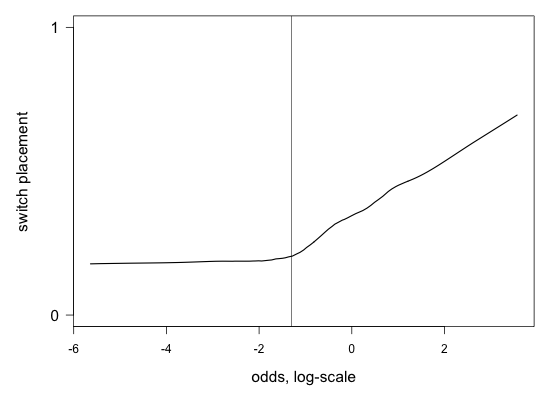
\includegraphics[scale=0.5]{figures/5-Figure_2.png}	
		\caption{The relationship between switch placement and odds (on the logarithmic scale). The values of 0 and 1 on the y-axis stand for switching within and outside the prepositional phrase, respectively.}
	\label{fig:5:2}
\end{figure}

\subsection{Frequency of the noun}

The facilitatory effect of word frequency in language production was already introduced in Chapter \ref{NP}. Following \citep[115]{macwhinney1997}, I argued that the associations between frequent words and the specific lexicogrammatical patterns with which they are usually used together may be stronger than such associations involving infrequent words. Under this view frequent words can trigger their lexicogrammatical patterns, including chunks, more easily than rare words. Conversely, lexicogrammatical patterns involving frequent words are more accessible than those involving rare lexemes. While in the previous chapter I analysed and evaluated the frequencies of both the adjectives and the nouns involved in the examined adjective-modified noun phrases, I restrict the analysis of frequency here to nouns because the prepositions under examination are all high-frequency items. 

In the context of the present chapter, frequent German nouns appearing in prepositional phrases, unlike rare nouns, are assumed to have a more pronounced ability to trigger, or co-activate, prepositions typically occurring with them. To test this hypothesis, frequencies of the nouns from the examined prepositional phrases were obtained from the deWaC corpus. \ref{tab:5:4} provides some of the prepositional phrases under investigation and the corresponding noun frequencies. The first five prepositional phrases include low-frequency nouns and exhibit phrase-internal switches, whereas the last five prepositional phrases include high-fre\-quen\-cy nouns and contain only embedded-language, i.e., German, elements.

\begin{table}
\begin{tabular}{lr}
		\lsptoprule
		PPs with switches placed within and outside the PP & \multicolumn{1}{c}{F\textsubscript{N}}\\\midrule
			v \textit{erotikshop} `to the sexshop' & 19\\
			na \textit{sporttag} `on a sports day' & 65\\
			s \textit{gummisohlen} `with rubber soles' & 80\\
			za \textit{einzimmerwohnung} `for a studio appartment' & 126\\
			v \textit{prüfungsstress} `under stress from exams' & 249\\
			\midrule
			\textit{nach hause} `(to) home' & 230408\\
			\textit{neben dem haus} `near the house' & 230408\\
			\textit{in der kirche} `in church' & 281589\\
			\textit{in die stadt} `to the city' & 480767\\
			\textit{am ende} `in the end' & 579078\\
		\lspbottomrule
	\end{tabular}
	\caption{Prepositional phrases switched inside and at the phrase boundary and the frequencies of the involved nouns, as measured in deWaC.\label{tab:5:4}}
\end{table}

\begin{figure}
    	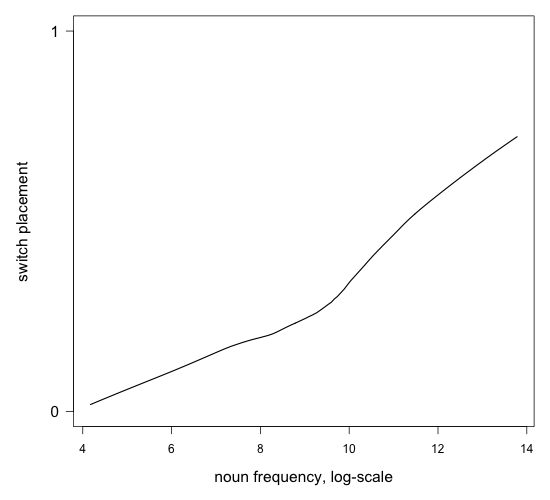
\includegraphics[scale=0.5]{figures/5-Figure_3.png}	
		\caption{The relationship between switch placement in the context of the prepositional phrase and the frequency of the noun (on the logarithmic scale).}
	\label{fig:5:3}
\end{figure}

The obtained frequency values were logarithmically transformed \citep[cf.][31]{baayen-analyzing}. The datum \textit{Erotikshop} `sex shop' was considered an outlier, due to its extremely low frequency in the corpus. The relationship between noun frequency and switch placement is plotted in \figref{fig:5:3}. The variable “switch placement” is on the vertical axis, and its values zero and one stand for a phrase-internal switch and a switch at the phrase boundary, respectively; noun frequency is on the horizontal axis. The Lowess curve demonstrates the effect of word frequency on switch placement: an increase in the noun frequency positively correlates with the tendency to switch the language at the phrase boundary. This is in line with the aforementioned hypothesis that the lexicogrammatical patterns involving high-frequency words are more accessible in production. Whether the frequency of the noun significantly contributes to predicting switch placement is tested in a regression model below.

\subsection{Word repetition}

The implicit memory effect of priming has been shown to affect monolingual language production in various domains of language (see \sectref{sec:var} for further details). In bilinguals, experimental studies have focused on cross-language priming effects in lexical access \citep{dijkstra-etal98, kroll-stewart94, vanhell-degroot98} and the production of syntactic constructions \citep{loebell-bock03, salamoura-williams06, schoonbaert-etal07}. Only recently has experimental research approached priming effects in bilingual speech. For example, \citep{kootstra-etal10} report that participants in their experiments tended to switch languages at the same position as in the prime sentence. This result, as \citeauthor{kootstra-etal12} report in their (2012) study, is driven by both the presence of cognates in the prime sentence and word repetition. In the conducted experiments, the subjects repeated a code-mixed sentence and then described a picture by using another code-mixed sentence. The authors show that lexical repetition between the prime sentence and the target picture, or the presence of a cognate in the prime and the target are capable of priming code-switches in sentences. Analyses of naturally occurring code-mixing have traditionally neglected priming effects, an exception to this trend is the work by \citep{torres-travis}. The authors have found that in the New Mexico Spanish-English Bilingual corpus, the distribution of syntactic structures in a specific syntactic context, namely, the expression of the Spanish first-person singular subject pronoun, largely depends on both language-internal and cross-language priming effects. We can conclude from these studies that repetition of words and structures in discourse should be given due consideration in analyses of naturally occurring bilingual speech. 

In the context of the prepositional phrase, an occurrence of a preposition in discourse can lead to a repeated selection of this preposition in subsequent discourse, provided that semantic compatibility is maintained. That is, once a preposition is produced, it is highly likely to be selected again in the same language, for instance:

\ea
\label{ex:5:14}
(LG05036)\\
\gll {priš-l-o-s'} {kogda} {\textsc{v}} \textit{lahr} {zaexa-l-i} {perv-ym} {del-om} {\textsc{v}} \textit{krankenhaus} {exa-t'}\\
	be.necessary-\textsc{pst-sg.n-refl} when to Lahr[\textsc{acc.sg.m}] come-\textsc{pst-pl} first-\textsc{instr.sg.n} thing-\textsc{instr.sg.n} to hospital[\textsc{acc.sg.m}] drive-\textsc{inf}\\
\glt `First thing when (they) came to Lahr, they had to drive to hospital.'
\z

\noindent The mixed prepositional phrase in (\ref{ex:5:14}) consists of the Russian preposition \textit{v} `to' and the German noun \textit{Krankenhaus} `hospital'. The speaker may alternatively have selected the German preposition \textit{in} `to' to produce the phrase \textit{ins Krankenhaus} `to hospital' (in this phrase the preposition-article combination \textit{in das} is usually realised as a contracted form). Nevertheless, the speaker selects the Russian preposition \textit{v} `in/to', which she produced as part of the string \textit{v Lahr} `to Lahr' in the previous clause. In other words, the first occurrence of the preposition \textit{v} appears to prime the use of the same lexical item with the German noun \textit{Krankenhaus} `hospital' in later discourse.

Nouns involved in the examined prepositional phrases also seem impervious to the pervasive effect of repetition priming, for instance:

\ea
\label{ex:5:15}
(LVa0510)\\
\gll {tam} \textit{\textsc{welle}} {na} {nix} {polete-l-a} {ili} {poli-l-a-s'} {nu} {i} {esli} {posmotr-et'} {čo} {tam} \textit{auf} \textit{der} \textit{\textsc{welle}} {vidno}\\ 
	{there} wave[\textsc{nom.sg}] onto 3\textsc{pl.acc} go.over-\textsc{pst-f.sg} or spout-\textsc{pst-f.sg-refl} \textsc{ptcl} and if look.at-\textsc{inf} what there on \textsc{art.dat.sg.f} wave visible\\
\glt `A wave went over them or spouted, and if you look at what is visible on the wave\dots{}'
\z

\noindent The noun from the inserted German prepositional phrase \textit{auf der Welle} `on the wave' in (\ref{ex:5:15}) appears in the prior discourse in the same language. Instead of repeating this lexical item in German in the subsequent prepositional phrase, the speaker may have produced the Russian equivalent \textit{volna} as well. Yet, the opposite is the case: the speaker uses the German noun \textit{Welle} persistently. The activation of this lexeme has presumably co-activated the German preposition \textit{auf} `on' associated with it. Furthermore, in the light of the analysis of example (\ref{ex:5:14}), according to which the choice of a specific preposition depends on its selection in the prior discourse, we could expect the Russian equivalent of this preposition, namely, \textit{na} `on', to occur rather than its German realisation, for the Russian preposition appears in the phrase \textit{na nih} `on(to) them' in the preceding clause. The result would have been a mixed phrase \textit{na Welle} `on the wave' (cf. Russian \textit{na volne}). A brief examination of possible motivations, or factors, underlying the choices among alternatives available to bilinguals makes evident that we cannot tell with certainty which of the considered motivations plays a decisive role in determining the speaker's choice to use a concrete alternative, unless we examine these motivations systematically and subject them to statistical tests.

The data were coded for the presence, or absence, of the examined prepositions and nouns in the window of eight seconds in the prior discourse (i.e., $5 \pm 3$ seconds, cf. \citealt[189]{szmrecsanyi2006}). The relationship between switch placement and word repetition in the same language is given in \figref{fig:5:4}. The upper panel concerns the repetition of prepositions and the lower panel refers to the repetition of nouns. As we can see in the upper panel, the proportion of prepositions repeated in mixed phrases is skewed; the asymmetry indicates the tendency to switching language within the prepositional phrase, given a prior occurrence of a specific preposition in the same language. The lower panel reveals relatively similar proportions of nouns that appear prior to the investigated German insertions. This observation demonstrates that noun repetition does not affect switch placement in the prepositional phrase in my bilingual corpus. Nevertheless, we cannot exclude an interaction between the repetition of a noun and the repetition of a preposition, especially as in the case of phrase repetition. For example:

\begin{figure}
	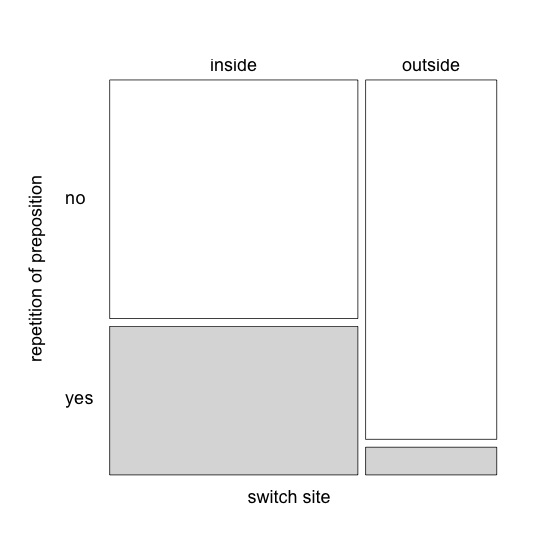
\includegraphics[scale=0.3]{figures/5-Figure_4a.png}	%[width=0.7\columnwidth]
	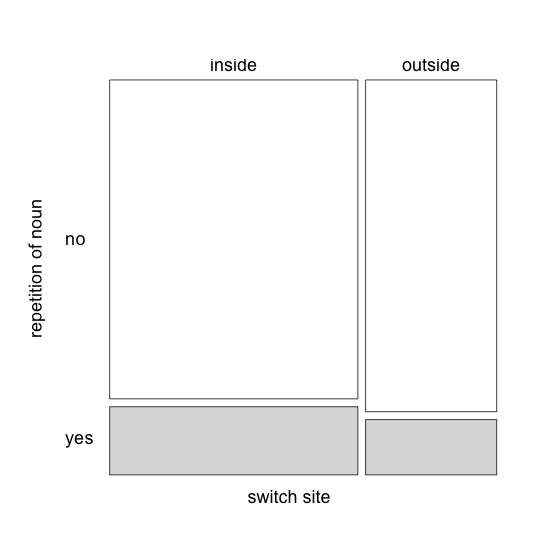
\includegraphics[scale=0.3]{figures/5-Figure_4b.png}	
		\caption{The relationship between switch placement and word repetition in the same language. The upper panel represents prior occurrences of target prepositions, the lower panel demonstrates prior occurrences of target nouns.}
	\label{fig:5:4}
\end{figure}

\ea
\label{ex5.16}
(HO1007)\\
\gll {ja} {im} {govor-ju} \itshape{wenn} \itshape{ich} \itshape{was} \itshape{von} \itshape{gott} \itshape{will} \itshape{geh-e} \itshape{ich} \itshape{\textsc{in}} \itshape{die} \itshape{kirche} {a} {oni} {mne} {nača-l-i} \itshape{\textsc{in}} \itshape{der} \itshape{kirche} {kak} {budto} {s} \textit{gott} {čë-to} {oni} {ne} {tak} {dela-jut} {čë} \textit{gott} {ime-et} {v} {vid-u}\\
	{\textsc{1sg.nom}} \textsc{3pl.dat} tell-\textsc{prs.1sg} if \textsc{1sg.nom} something from god want.\textsc{prs.1sg} go.\textsc{prs-1sg} \textsc{1sg.nom} to \textsc{art.acc.sg} church but \textsc{3pl.nom} \textsc{1sg.dat} begin-\textsc{pst-pl} in \textsc{art.dat.sg} church as if with god[\textsc{?sg}] something.\textsc{acc} \textsc{3pl.nom} \textsc{neg} so do-\textsc{prs3pl} what.\textsc{acc} god$[$\textsc{nom.sg}$]$ have-\textsc{prs3sg} in view-\textsc{loc.sg}\\
\glt `I tell them, if I want something from God, I go to church, but they began like, in church people do not treat God as he intends them to.'
\z

\noindent Here, the phrase \textit{in die Kirche} `to church' appears in a German clause for the first time and is then echoed in a mixed clause, albeit with the article in a different case. Although this kind of repetition is relatively rare, an interaction between the variables “repetition of preposition” and “repetition of noun” would be able to account for this example. In most cases, however, occurrences of prepositions in the prior discourse affect the choice of the preposition in the target phrase. In other words, prepositions seem to be stronger primes than nouns.

To summarise, I have shown thus far that four factors are predictive of switch placement in the context of the prepositional phrase: (\textit{i}) the odds based on the frequency with which prepositions and nouns appear together, (\textit{ii}) the frequency of the noun, (\textit{iii}) the presence, or absence, of prepositions in the same language in the prior discourse and (\textit{iv}) the presence, or absence, of nouns in the prior discourse, albeit only when used with the repeated preposition. As detailed above, instances such as (\ref{ex:5:15}) cannot be attributed to a single factor. This circumstance necessitates examining the pertinent factors as potential determinants of the scrutinised variation by means of a statistical test, which would simultaneously take account of the factors as well as their interactions.

\section{Statistical prediction of switch placement}

\noindent The aim of this section is to investigate the factors described above as they compete and interact with one another while conditioning switch placement in the prepositional phrase. Addressing the issues of competition and interaction entails a number of questions: How predictive is noun frequency of switch placement, all things being equal? Which factor is the most important predictor of the observed variation? Do individual preferences for switch placement override the regularity of the identified linguistic tendencies? Like \sectref{4:stat}, this chapter investigates these issues by using the generalised linear mixed model. Probabilities of binary outcomes -- a switch within a prepositional phrase and a switch at the boundary of a prepositional phrase -- will be determined on the basis of the predictor variables, i.e., the factors analysed above. Significant interactions between the dependent variable “switch placement” and the predictor variables will provide objective evidence of the relevance of each of the predictors.

\subsection{Model fitting}

In order to obtain a minimal adequate regression model, the common procedure \citep{baayen-2013,szmrecsanyi-2013} was employed, which is as follows. The maximal model contained the four factors considered above as main effects: the odds, based on the frequency with which the examined nouns are used with prepositions; the frequency of the involved noun; the prior occurrences and non-occurrences of the target noun; and the prior occurrences and non-occurrences of the target preposition. The maximal model also included interactions between these factors. The speakers' individual differences in mixing behaviour -- a propensity to insert German nouns into Russian prepositional phrases or, rather, a predilection for maintaining the integrity of the phrase  --  may alter the tendencies determined solely by the fixed factors. These individual differences are considered in the random variable “speaker”. A random effect for the variable “item” could not be included owing to its high variability, namely, 197 various lexemes appear in the 244 prepositional phrases under analysis. The model was thus run without the by-item random variable. The model simplification procedure consisted in the omission of the factors and interaction terms that added no significant explanatory power to the model. According to \citet[281]{baayen-analyzing}, the calculation of the \textit{C} index of concordance is the basis for estimating the explanatory power of main effects and interaction terms. The process of model reduction resulted in the exclusion of the following interaction terms from the model: noun frequency $\times$ odds and prior noun $\times$ noun frequency. Subsequently, the inclusion of the by-subject random effect was justified by the estimation of the \textit{C} index of a generalised linear model without random effects. The model that included the random factor appeared to perform significantly better than the model without a random effect (which is in line with established practice in similar cases, cf. \citealt{bresnan-etal}; \citealt{tagliamonte-baayen-2012}). The final, minimal adequate model is presented in Table \ref{tab:5:5}.

\begin{table}
\begin{tabular}{l rrl l}
		 \lsptoprule
	     Factor & Odds & \multicolumn{1}{c}{Est.} & \multicolumn{1}{c}{$\text{Pr}(>|z|)$}  &\\\midrule
		(Intercept) & 0.012 & −4.427  & 0 & ***\\
		Prior preposition & 0.030 & −3.496 & 0 & ***\\
		Prior noun & 0.440 & −0.820 & 0.178 & \\ 
		Noun frequency & 1.568 & 0.449 & 0 & ***\\
		Log odds & 1.359 & 0.307 & 0.001 & **\\
		Prior preposition $\times$ prior noun & 24.753 & 3.209 & 0.007 & **\\  \midrule
		\multicolumn{5}{l}{Random effect:}\\
		\multicolumn{5}{l}{Speaker}\\
		\multicolumn{5}{l}{(intercept, $N = 19, \text{variance} = 0.915, \sigma = 0.956$)}\\
		\midrule
		\multicolumn{2}{l}{Summary statistics:}\\
		\multicolumn{2}{l}{$N$} &  244\\
		\multicolumn{2}{l}{\% correct predictions (\% baseline)}  & 84 (69)\\
		\multicolumn{2}{l}{\textit{C} index of concordance}  & 0.871\\
		\multicolumn{2}{l}{Somer's Dxy} &  0.742\\
		\lspbottomrule
\end{tabular}
	\caption{Predicting switch placement in the context of the prepositional phrase: minimal adequate generalised linear mixed model. Predicted odds ratios are for switches placed at the phrase boundary. Significance codes: *significant at $p < 0.05$, ** $p < 0.01$, *** $p < 0.001$.\label{tab:5:5}}
\end{table}

\subsection{Model evaluation and model discussion}

\noindent The minimal adequate model reported in Table  \ref{tab:5:5} is of high quality. The model correctly predicts 84\% of all instances of switch placement in the data set, while the categorical prediction of switch placement by always guessing a switch placed within the prepositional phrase will be correct in 69\% of all cases. The \textit{C} index of concordance between the predicted probability and the observed binary outcomes is 0.871, which indicates that the model has high predictive power. The performance indicator Somers' D$_{xy}$, a rank correlation coefficient between predicted probabilities and observed binary response, is 0.725, which again signals the model’s high predictive capacity. Regarding the random effect for the variable “speaker”, we can conclude from its estimated variance and standard deviation that the variation among speakers, although minor, still contributes to the distribution of the examined data.

The main effects in the model provide positive evidence for the assumptions formulated above. The signs of the regression coefficients (Estimates) in Table \ref{tab:5:5} reveal the direction of the adjustment to the intercept. Hence, a prior occurrence of the target preposition and that of the target noun condition the placing of the switch between the preposition and the noun, whereas both odds, based on co-occurrence frequency, and noun frequency favour switching at the phrase boundary. Consider the odds ratios reported in Table \ref{tab:5:5}. Among the fixed-effect factors, repetition of the preposition has the largest effect size, which means that if the target preposition appears in the prior discourse, the likelihood of switching the language at the phrase boundary decreases by 97\%. That is, there is a high probability that the previously occurring preposition will be selected in the target prepositional phrase. The interaction between a prior occurrence of the target preposition and that of the target noun in the discourse is another strong effect: If both the preposition and the noun appear in the preceding discourse, the odds for switch placement at the phrase boundary increase by a factor of approximately 25. This interaction term accounts for the case illustrated by example (\ref{ex:5:15}). But when the occurrences of the noun and the preposition in the prior discourse do not interact, both of them favour switch placement within the prepositional phrase. Although the predictor “prior occurrence of noun” does not attain statistical significance, it interacts with the factor “prior occurrence of preposition”, enhancing the model's predicative capacity. This is the main reason for retaining this predictor in the minimal adequate model. Moreover, this interaction reaches a high level of statistical significance.

After considering the effect sizes of the factors contributing to the minimal adequate model, it is necessary to discuss these factors’ overall importance. This parameter is visualised in \figref{fig:5:5} by plotting the decrease in the Akaike Information Criterion (AIC) of the model if a factor is removed from the minimal model. According to \citet{szmrecsanyi-2013}, more sizable decreases in the AIC criterion of a factor stand for its increased overall importance. In predicting switch placement in the context of 244 prepositional phrases from the data set, the most important factor is “prior occurrence of the target preposition”. Noun frequency is the second most relevant predictor, followed by “(log) odds”, which is based on the measured co-occurrence frequency. The model's Akaike Information Criterion sinks drastically when the factor “noun frequency” is removed from the model. The extent of this decrease appears to substantially exceed the extent of the decrease of factor “(log) odds”. The interaction between the prior occurrence of the noun and that of the preposition is ranked last. The prior occurrence of the noun is not among the plotted factors owing to its low level of importance for the model, when included without an interaction term.

\begin{figure}
	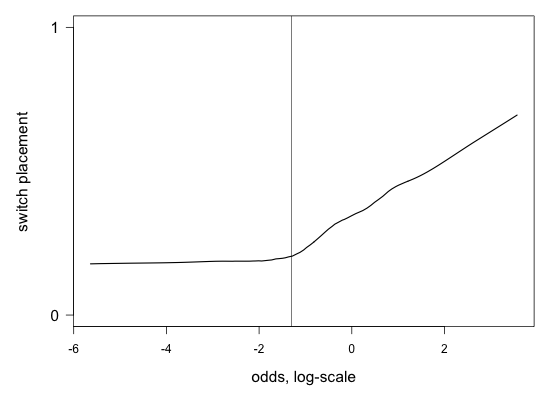
\includegraphics[scale=0.5]{figures/5-Figure_2.png}	
	\caption{Importance of factors in model: decrease in Akaike Information Criterion (AIC) if factor removed. (The table representation is based on \citealt{szmrecsanyi-2013}.)}\label{fig:5:5}
\end{figure}

A somewhat surprising result of the minimal adequate model is that the predictor “noun frequency” is more important in accounting for variation in the data than the factor “(log) odds”, which is a measure of competition among co-occurrences of nouns and prepositions. A question arises as to why “(log) odds” is a less important predictor than “noun frequency”. Although “(log) odds” is the only factor that takes preposition-noun co-occurrences into consideration, we cannot rule out the possibility that it  performs in the model inadequately. A possible reason for this under-performance is the severe competition among chunks involving high-frequency nouns. As these nouns combine with several prepositions at high rates, the joint frequency of such combinations are likely to prevail over the frequency of a particular preposition-noun combination in focus. In other words, the higher the frequency of the noun, the larger the number of its collocates, usually referred to as “family size”, and the more difficult it is for a specific combination to come out on top of the distribution and become selected in production. \tabref{tab:5:6} provides an illustration of these intricacies. 

\begin{table}
	\begin{tabular}{lr}
		\lsptoprule
		Co-occurring prepositions & Frequency of co-occurrence\\\midrule
		\textit{an} `at' & 157220 \\
		\textit{zu} `to' & 67684 \\
		\textit{bis} `by' & 22152 \\
		\textit{nach} `after' & 18279 \\
		\textit{gegen} `towards' & 14240 \\
		\textit{seit} `since' & 13063 \\
		\textit{von} `from' & 7214 \\
		\textit{vor} `before' & 6993 \\
		\textit{ohne} `without' & 5242 \\
		\textit{mit} `with' & 5153 \\
		\textit{für} `for' & 3824 \\
		\textit{ab} `from' & 3398 \\
		\textit{auf} `to' & 2408 \\
		\lspbottomrule
	\end{tabular}
	\caption{Prepositions co-occurring with the German noun \textit{Ende} `end' and their respective co-occurrence frequencies.\label{tab:5:6}}
\end{table}


\tabref{tab:5:6} presents a set of prepositions co-occurring with the high-frequency noun \textit{Ende} `end'. As this noun combines with an array of prepositions at high rates, we may describe the competition among the thirteen prepositions as stiff. The preposition \textit{an} `at' accounts for the lion's share in the overall distribution of the [P -- \textit{Ende}] pattern. In fact, it is this preposition which the speaker selects. However, the summated frequencies of the noun's remaining companions outbalance the frequency of the competition winner \textit{an} `at'. As a result, the top collocate's odds value is lower than 1. It is noteworthy that the other high-frequency nouns in the data set are also affected. We can thus contend that instead of exerting a direct influence on switch placement, noun frequency may act as a leverage for combinations of prepositions and high-frequency nouns.  

To summarise, in this section I have demonstrated that frequency-based factors, such as “noun frequency” and “odds”, based on co-occurrence frequency, as well as the processing-related factor “word repetition (priming)” effectively predict switch placement in the context of the prepositional phrase. Speaker variation in switching the language at the phrase boundary or within the phrase was found to be marginal.

\section{Conclusions and discussion}

This chapter has explored variation in switch placement in the prepositional phrase in Russian-German code-mixing as an outcome of factors related to intricacies of language use in terms of the speakers’ experience with language as such, i.e., in the global sense, and their sensitivity to the use of linguistic elements in the immediately preceding discourse, i.e., at the local level. Specifically, it has focused on the role of factors such as word frequency, competition among multiword strings varying in usage frequency, and recency of a word in the discourse. Additionally, I have shown that a combination of corpus-linguistic, computational and statistical methods proves to be useful for analyses of variation in code-mixing patterns.

The principal findings of the study include two frequency effects: First, frequencies with which prepositions and nouns co-occur influence switch placement in the context of the prepositional phrase. If a noun and a specific preposition appear together more frequently than all the other combinations of this noun with prepositions, a switch between this noun and the given preposition is unlikely. Conversely, if the frequency of co-occurrence of a noun and a specific preposition is low, the chance for a switch to be placed within the prepositional phrase is high. The fact that high-frequency preposition-noun combinations are impervious to phrase-internal switching is explained in terms of their holistic representation in the speakers' mental lexicon. Whenever two or more items co-occur on a regular basis in one of the languages involved in code-mixing, speakers store and retrieve these multiword sequences from memory as units, and their production becomes automatised (cf. Chapter \ref{UBL}). This finding accounts for embedded-language islands as word strings welded together in language usage. Similar to the results reported in Chapter \ref{NP}, it  corroborates Backus’ (\citeyear{backus-units-2003}) unit hypothesis. The competition among multiword strings structured as prepositional phrases was modelled by (log) odds. 

Another finding concerns a strong correlation between the frequency of the nouns involved in the examined prepositional phrases and switch placement. As reported above, German high-frequency nouns are accompanied by German prepositions in mixed sentences more often than by Russian prepositions. That is, the speakers switch the language to German at the phrase boundary in this case. I have argued that this tendency is due to the fact that high-frequency nouns usually form several recurrent multiword strings with various prepositions. The stiff competition among these strings is likely to weaken the predictive capacity of the competition measure odds. As a result, the frequency of the noun appears to be a more important predictor of the variation in the data than the odds. However, as stated above, the influence of noun frequency on switch placement may be indirect. Interestingly, in the context of the adjective-modified noun phase (cf. Chapter \ref{NP}), noun frequency appeared to exert no significant influence on the variation in the mixing patters. Another interpretation of the noun frequency effect pertains to the accessibility of high-frequency nouns and their lexicogrammatical patterns, including multiword chunks, in production. Being extremely accessible, these nouns may easily co-activate the contexts in which they typically occur. \citet{arnon-snider} have presented evidence of a similar effect in language comprehension. 

The statistical analysis conducted reveals that the most important predictor of switch placement in the examined context is a prior occurrence of the preposition in the prior discourse. The chances for producing the preposition in one of the involved languages are higher if this preposition also occurs in the same language during the previous eight seconds of discourse, provided that semantic compatibility is maintained. The occurrence of the preposition in the prior discourse, which is usually framed by the matrix language Russian, has, in most cases, the use of the Russian preposition in the target phrase, or placing the switch within the prepositional phrase. This recency effect is so strong that it overrules the effects of frequency discussed above. This tendency can be attributed to the following factors: First, the investigated prepositions are distinguished by high usage frequencies, and are extremely polysemous (the data set includes no secondary prepositions). Apparently, their polysemous nature and frequent use are interdependent. Second, like pronouns, which are the focus of analysis in \citep{torres-travis}, prepositions are function words and seem to go unnoticed in language production. That is, function words appear to be stronger primes than content words. Third, code-mixing occasionally co-occurs with self-repair, in which case part of the lexical material remains preserved in the target structure, as in the example below.

\ea
\label{ex:5:17}
(LR0316)\\
\gll \itshape{stra-} \itshape{stra{ß}e(n)bahn} {priezža-l} {v} {dvadcat'} {četyre} {minut-y} {v(.)} \textit{also} {v} \textit{einundzwanzig} {dvadcat'} {četyre}\\
	{} {tram$[$\textsc{nom.sg}$]$} arrive-\textsc{pst.m.sg} at twenty four minute-\textsc{gen.sg} at \textsc{ptcl} at twenty-one twenty four\\
\glt `The tram arrived at twenty-four minutes, well, at nine twenty-four.'
\z

\noindent The preposition \textit{v} `at' appears before the mixed phrase \textit{v einundzwanzig dvadcat' četyre} `at twenty-one twenty-four' in an instance of self-repair, but also earlier, at the beginning of the utterance. 

Future work should therefore include follow-up research designed to examine patterns of code-mixing with regard to self-repair as well as repetition priming. An important question for future studies is to elucidate the role of noun frequency for switching preferences in the prepositional phrase and to develop and test other models of competition among functionally and structurally similar word strings. 

The findings presented in this chapter parallel the results reported in Chapter \ref{NP} in that in the prepositional phrase as well as in the adjective-modified noun phrase, the choice between producing a mixed constituent and inserting an embedded-language island, appears to depend on the frequency of the linguistic material and its accessibility in the memory, referred to as recency in discourse and repetition priming. This chapter has also shown that in addition to usage frequency, the choice is influenced by the competition among the prepositions occurring with a specific noun at varying rates. In situations in which a clear winner is identifiable, the probability of selecting the string with this preposition is extremely high. 

The difference between the distribution of the mixing patterns in the prepositional phrase and in the adjective-modified noun phrase pertains to the nature of the elements involved. While the latter syntactic context is determined by open-class words, the syntactic context in the present chapter involves combinations of open-class and closed-class words. As mentioned in Chapter \ref{NP}, the selection of nouns is an unconstrained process \citep{boumans-syntax-1998}, whereas the selection of adjectives is less unconstrained (e.g., German attributive adjectives never modify Russian nouns). As to the selection of  prepositions, the options are much more restricted. Of the analysed nouns, the majority regularly occurs with a handful of prepositions. That is, the choice between a Russian, and a German preposition is conditioned by the limited size of the available inventories. Against this background, it would be interesting to explore the selection of elements in a context permitting choices among even fewer alternatives. Regarding the competition among the available options, we may assume that it will be much stronger owing to a reduced number of competing candidates. It well may be that in this situation, frequency will play even a more crucial role in conditioning the mixing patterns. One context which allows us to investigate variation in mixing patterns involving a small inventory of elements is plural marking. In this context, embedded-language nouns in sentences framed by the matrix language either receive  matrix language plural markers, or retain their embedded-language plural markers. It is to this study that I turn in the next chapter.

%\begin{figure} 

%\begin{forest} 
%[ {mixed PPs\\456 (100 \%)}
%[{alternation\\25 (5.5 \%)}]
%[insertion 
%    [ {ML: Russian} 
%       [{adjacent insertion\\18 (4.0 \%)}]
%        [{lone insertion} 
%            [{simple\\333 (73.1 \%)}] 
%            [{with an expanded NP\\71 (15.4 \%)}] 
%                ] 
%                ] 
%    [{ML: German\\9 (2.0 \%)}] 
%    ]
%]
%\end{forest}
%\centering
%\caption{\textit{Prepositional phrases involved in code-mixing: variability of structures and proportions.}}\label{fig:5:1}
%\end{figure}
